% opsph.tex
% opérateurs sphériques sur la sphère

\chapter{Approximation des opérateurs sphériques sur la Cubed-sphere}

La résolution des équations de type Shallow-Water \REF la sphère $\mathbb{S}_a^2$ demande le calcul approché d'opérateurs classiques. Les opérateurs différentiels sont indispensables pour la discrétisation spatiale. On pense en particulier aux opérateurs divergence, gradient ou rotationnel. Dans cette section, nous les définissons sur la Cubed-sphere. 
Nous avons vu dans le cas 1D qu'un opérateur de filtrage peut être utile pour supprimer les modes de type "$+1/-1$" qui perturbent le calcul lors de la discrétisation en temps. Nous définissons les opérateurs de filtrages permettant d'aboutir au filtrage qui sera utilisé dans la discrétisation temporelle des équations.
Dans ce chapitre, les notations employées telles que $\xi$, $\eta$, $\alpha$, ... sont celles employées dans le chapitre \REF concernant la Cubed-sphere.

\section{Opérateurs différentiels sur la Cubed-sphere}

\subsection{Définition des opérateurs}
Soit $\mathbf{x}_{i,j}^k$ un point de la Cubed-sphere avec $- N/2 \leq i,j \leq N/2$ et $k = (I) \cdots (VI)$. Alors il existe deux grands cercles $C_i^{(1)}$ et $C_j^{(2)}$ deux grands cercles tels que $\mathbf{x}_{i,j}^k \in C_i^{(1)} \cap C^{(2)}_j$. $\alpha$ et $\beta$ sont respectivement les angles paramétrant $C_i^{(1)}$ et $C_j^{(2)}$.

On a définit le gradient en $\mathbf{x}_{i,j}^k$ par 
\begin{equation}
\nabla_T h = \dfrac{\partial h}{\partial \alpha}_{|C^{(2)}_j} \mathbf{g}^{\alpha} + \dfrac{\partial h}{\partial \beta}_{|C^{(1)}_i} \mathbf{g}^{\beta},
\end{equation}
où $h \mathbf{x} \in \mathbb{S}_a^2 \mapsto h(\mathbf{x})$ est une fonction régulière sur la sphère.

Le cercle $C_i^{(1)}$ (resp. $C_j^{(2)}$) est une isocline $\xi = \xi_i$ (resp $\eta = \eta_j$) constant. D'après le théorème \eqref{th:gradient_xieta}, le gradient est calculable via la formule
\begin{equation}
\nabla_T h = \dfrac{\partial h}{\partial \xi}_{|\eta_j} \mathbf{g}^{\xi} + \dfrac{\partial h}{\partial \eta}_{|\xi_i} \mathbf{g}^{\eta}.
\end{equation}
On remarque que si l'on est capable de calculer les dérivées partielles $\partial_{\xi}$ et $\partial_{\eta}$ le long des grands cercles, alors on est capable de déterminer la valeur du gradient.

Soit $\mathbf{v} : \mathbf{x} \in \mathbb{S}_a^2 \mapsto \mathbf{v}(\mathbf{x}) \in \mathbb{T}_{\mathbf{x}} \mathbb{S}_a^2$ un champ de vecteur tangent à la sphère. On définit dans un premier temps la \textit{divergence} et le \textit{rotationnel} de $\mathbf{v}$ notés $\nabla_T \cdot \mathbf{v}$ et $\nabla_T \wedge \mathbf{v}$.

\begin{definition}
Soit $\mathbf{v} : \mathbf{x} \in \mathbb{S}_a^2 \mapsto \mathbf{v}(\mathbf{x}) \in \mathbb{T}_{\mathbf{x}} \mathbb{S}_a^2$ un champ de vecteur régulier sur la sphère. Alors la divergence de $\mathbf{v}$ en $\mathbf{x} \in C_i^{(1)} \cap C_j^{(2)}$ est donnée par
\begin{equation}
\nabla_T \cdot \mathbf{v} = \dfrac{\partial \mathbf{v}}{\partial \alpha}_{|C^{(2)}_j} \cdot \mathbf{g}^{\alpha} + \dfrac{\partial \mathbf{v}}{\partial \beta}_{|C^{(1)}_i} \cdot \mathbf{g}^{\beta}.
\end{equation}
\label{def:divergence}
La notation $\cdot$ désigne le produit scalaire usuel dans $\mathbb{R}^3$.
\end{definition}
Le rotationnel d'un champ de vecteurs représente la tendance des lignes de courant de $\mathbf{v}$ à tourner autour d'un point. Il est définit par

\begin{definition}
Soit $\mathbf{v} : \mathbf{x} \in \mathbb{S}_a^2 \mapsto \mathbf{v}(\mathbf{x}) \in \mathbb{T}_{\mathbf{x}} \mathbb{S}_a^2$ un champ de vecteur régulier sur la sphère. Alors le rotationnel de $\mathbf{v}$ en $\mathbf{x} \in C_i^{(1)} \cap C_j^{(2)}$ est donnée par
\begin{equation}
\nabla_T \wedge \mathbf{v} =  \mathbf{g}^{\alpha} \wedge \dfrac{\partial \mathbf{v}}{\partial \alpha}_{|C^{(2)}_j} + \mathbf{g}^{\beta} \wedge \dfrac{\partial \mathbf{v}}{\partial \beta}_{|C^{(1)}_i}
\end{equation}
où $\wedge$ désigne le produit vectoriel.
\label{def:rotationnel}
\end{definition}
La \textit{vorticité} du champ de vecteurs $\mathbf{v}$ est la composante normale du rotationnel :
\begin{equation}
\vort ( \mathbf{v} ) = \left( \nabla_T \wedge \mathbf{v} \right) \cdot \mathbf{k}
\label{eq:vorticité}
\end{equation}
avec $\mathbf{k}$ le vecteur unitaire extérieur à la sphère en $\mathbf{x} \in \mathbb{S}_a^2$, il vérifie l'égalité
\begin{equation}
\mathbf{k} = \dfrac{1}{a} \mathbf{x}.
\end{equation}

En utilisant la proposition \ref{prop: g_alpha g_beta fct de g_xi g_eta}, il est facile de montrer que des égalités permettant de calculer les opérateurs à l'aide des dérivées en $\xi$ et en $\eta$.

\begin{theoreme}
Soit $h : \mathbf{x} \in \mathbb{S}_a^2 \mapsto h(\mathbf{x})$ une fonction régulière et $\mathbf{v} : \mathbf{x} \in \mathbb{S}_a^2 \mapsto \mathbf{v}(\mathbf{x}) \in \mathbb{T}_{\mathbf{x}} \mathbb{S}_a^2$ un champ de vecteurs régulier. Alors en $\mathbf{x}_{i,j}^k$ un point de la Cubed-Sphere, les égalités suivantes sont satisfaites :
\begin{itemize}
\item \textbf{Gradient} :
\begin{equation}
\nabla_T h = \dfrac{\partial h}{\partial \xi}_{|\eta_j} \mathbf{g}^{\xi} + \dfrac{\partial h}{\partial \eta}_{|\xi_i} \mathbf{g}^{\eta},
\end{equation}

\item \textbf{Divergence} :
\begin{equation}
\nabla_T \cdot \mathbf{v} = \dfrac{\partial \mathbf{v}}{\partial \xi}_{|\eta_j} \cdot \mathbf{g}^{\xi} + \dfrac{\partial \mathbf{v}}{\partial \eta}_{|\xi_i} \cdot \mathbf{g}^{\eta},
\end{equation}

\item \textbf{Rotationel} :
\begin{equation}
\nabla_T \cdot \mathbf{v} = \mathbf{g}^{\xi} \wedge \dfrac{\partial \mathbf{v}}{\partial \xi}_{|\eta_j} + \mathbf{g}^{\eta} \wedge \dfrac{\partial \mathbf{v}}{\partial \eta}_{|\xi_i}.
\end{equation}
\end{itemize} 
\end{theoreme}

Pour calculer une valeur approchée des opérateurs gradient, divergence et rotationnel aux points du maillage de la Cubed-Sphere, il faut calculer une valeur approchée de la dérivée d'une fonction le long d'un grand cercle. C'est à dire, calculer $f_{\xi,i,j}$ et $f_{\eta,i,j}$ tels que 
\begin{equation}
\left\lbrace
\begin{array}{rl}
f_{\xi,i,j} \rightarrow \partial_{\xi} f ( \mathbf{x}_{i,j}^k) & \text{ lorsque } \Delta \xi \rightarrow 0\\
f_{\eta,i,j} \rightarrow \partial_{\eta} f ( \mathbf{x}_{i,j}^k) & \text{ lorsque } \Delta \eta \rightarrow 0
\end{array}
\right.
\end{equation}
La section suivante consiste à détailler une procédure pour calculer ces dérivées partielles approchées et à déterminer l'erreur effectuée lors du calcul.





\subsection{Approximation de dérivées sur les grands cercles}

On pose $f : \mathbf{x}\in \mathbb{S}_a^2 \mapsto f(\mathbf{x})$ la fonction que l'on souhaite dérivée le long des grands cercles aux points du maillage de la Cubed-Sphere.
Si $\mathbf{x}_{i,j}^k$ est un point de la Cubed-Sphere avec $k = (I) \cdots (VI)$, ainsi que $-N/2 \leq i,j \leq N/2$. On souhaite calculer une valeur approchée de 
$
\partial_{\xi} f (\mathbf{x}_{i,j}^k) \text{ et } \partial_{\xi} f (\mathbf{x}_{i,j}^k)
$.
On suppose par exemple $k = (I)$ mais la méthode est la même sur les autres panels. Alors il existe deux grands cercles de la Cubed-Sphere $C_i^{(1)}$ et $C_j^{(2)}$ tels que 
\begin{equation}
\mathbf{x}_{i,j}^k \in C_i^{(1)} \cap C^{(2)}_j.
\end{equation}
$C^{(1)}_i$ est une isoligne en $\xi = \xi_i$ constant et $C^{(2)}_j$ est une isoligne en $\eta = \eta_j$ constant.
Pour calculer une valeur approchée de $\partial_{\xi} f (\mathbf{x}_{i,j}^{(I)})$, on souhaite connaître toutes les valeurs de $f$ aux points équirépartis le long du cercle $C^{(2)}_j$. On pose $\mathbf{m}_p$ avec $0 \leq p \leq 4N-1$ les points de $C^{(2)}_j$ construits de la manière suivante :
\begin{itemize}
\item si $0 \leq p \leq N$ alors $\mathbf{m}_p = \mathbf{x}^{(I)}_{p-N/2,j}$, il s'agit des points du cercle $C^{(2)}_j$ associés au panel $(I)$ sur le maillage. Ils sont représentés par des ronds bleus sur les figures \ref{fig:patron_cs} et \ref{fig: panel II_interp},
\item si $N+1 \leq p \leq 2N-1$ alors les points ne font pas partis du maillages. Il s'agit des des points d'intersections de $C^{(2)}_j$ avec les isoligne $\xi = \xi_i^{(II)}$ du panel $(II)$. C'est à dire l'intersection de $C^{(2)}_j$ avec les cercles de $(II_{\beta})$. Ces points sont représentés par les carrés bleus dans les figures \ref{fig:patron_cs} et \ref{fig: panel II_interp}. Les coordonnées de ces points ont été calculées dans la partie \REF.
\item si $2N \leq p \leq 3N$ alors $\mathbf{m}_p = \mathbf{x}^{(III)}_{p-3N/2}$. Il s'agit des points de la Cubed-Sphere du panel $(III)$ représentés par des ronds bleus sur la figure \ref{fig:patron_cs},
\item si $3N+1 \leq p \leq 4N-1$ alors $\mathbf{m}_p$ est constitués des points d'intersections de $C^{(2)}_j$ avec les cercles de $(IV_{\beta})$. Il ne s'agit pas de points de la grille. Ces points sont représentés par les carrés bleus dans la figure \ref{fig:patron_cs}.
\end{itemize}

\begin{figure}
\begin{center}
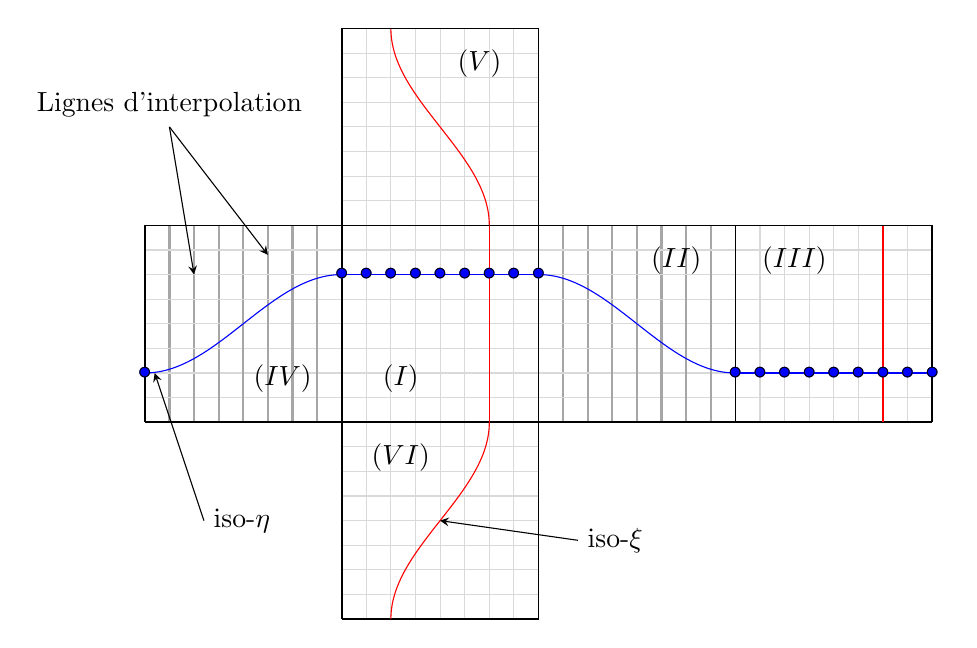
\begin{tikzpicture}[scale=2.5]
	\foreach \x in {1,...,7}
		{ \draw [color=gray!70, line width=0.8pt] (0.125*\x,1) -- (0.125*\x,2) ;
		\draw [color=gray!30] (0,1+0.125*\x) -- (1,1+0.125*\x) ;
		\draw [color=gray!30] (1+0.125*\x,1) -- (1+0.125*\x,2) ;
		\draw [color=gray!30] (1,1+0.125*\x) -- (2,1+0.125*\x) ;
		\draw [color=gray!70, line width=0.8pt] (2+0.125*\x,1) -- (2+0.125*\x,2) ;
		\draw [color=gray!30] (2,1+0.125*\x) -- (3,1+0.125*\x) ;
		\draw [color=gray!30] (3+0.125*\x,1) -- (3+0.125*\x,2) ;
		\draw [color=gray!30] (3,1+0.125*\x) -- (4,1+0.125*\x) ;
		\draw [color=gray!30] (1+0.125*\x,0) -- (1+0.125*\x,1) ;
		\draw [color=gray!30] (1,0.125*\x) -- (2,0.125*\x) ;
		\draw [color=gray!30] (1+0.125*\x,2) -- (1+0.125*\x,3) ;		
		\draw [color=gray!30] (1,2+0.125*\x) -- (2,2+0.125*\x) ;
		}
	

	\draw [line width=0.6pt] (1,3) -- (2,3) ; 
	\draw [line width=0.6pt] (0,2) -- (4,2) ; 	
	\draw [line width=0.6pt] (0,1) -- (4,1) ; 
	\draw [line width=0.6pt] (1,0) -- (2,0) ; 
	
	\draw [line width=0.6pt] (0,2) -- (0,1) ;
	\draw [line width=0.6pt] (1,3) -- (1,0) ;
	\draw [line width=0.6pt] (2,3) -- (2,0) ;
	\draw [line width=0.6pt] (3,2) -- (3,1) ;
	\draw [line width=0.6pt] (4,2) -- (4,1) ; 
	
	\draw (0.7,1.1) node[above]{$(IV)$} ; 
	\draw (1.3,1.1) node[above]{$(I)$} ; 
	\draw (2.7,1.7) node[above]{$(II)$} ;
	\draw (3.3,1.7) node[above]{$(III)$} ;  
	\draw (1.7,2.7) node[above]{$(V)$} ;  
	\draw (1.3,0.7) node[above]{$(VI)$} ; 
	
	\draw [samples=100,domain=0:1,color=blue] plot({\x},{1.5-(2*0.125)*cos(180*\x)});
	\draw [samples=100,domain=1:2,color=blue] plot({\x},{1.5+2*0.125});
	\draw [samples=100,domain=1:2,color=blue] plot({\x+1},{1.5-2*0.125*cos(180*\x)});
	\draw [samples=100,domain=3:4,color=blue] plot({\x},{1.5-2*0.125});
	\draw [>=stealth, <-] (0.05,1.25) -- (0.3,0.5) ;
	\draw  (0.3,0.5) node[right] {iso-$\eta$} ;
	
	\draw [samples=100,domain=0:1,color=red] plot({1.5-2*0.125*cos(180*\x)},{\x});
	\draw [samples=100,domain=1:2,color=red] plot({1.5+2*0.125},{\x});
	\draw [samples=100,domain=1:2,color=red] plot({1.5-2*0.125*cos(180*\x)},{\x+1});
	\draw [samples=100,domain=1:2,color=red] plot({4-2*0.125},{\x});
	\draw [>=stealth, <-] (1.5,0.5) -- (2.2,0.4) ;
	\draw  (2.2,0.4) node[right] {iso-$\xi$} ;
	
	\draw  (0,1+2*0.125) node[color=blue] {$\bullet$} ;
	\draw (0,1+2*0.125) node {$\circ$} ;
	
	\foreach \k in {0,...,8}
		{\draw  (1+0.125*\k,1.5+2*0.125) node[color=blue] {$\bullet$} ;
	   	\draw (1+0.125*\k,1.5+2*0.125) node {$\circ$} ;
	   	\draw  (3+0.125*\k,1+2*0.125) node[color=blue] {$\bullet$} ;
	   	\draw (3+0.125*\k,1+2*0.125) node {$\circ$} ;
	   	}
	   	
	\foreach \x in {1,...,7}
		{\draw  ({0.125*\x},{1.5-2*0.125*cos(180*0.125*\x)}) node[color=blue] {\begin{tiny}$\blacksquare$\end{tiny}} ;
	   	\draw ({0.125*\x},{1.5-2*0.125*cos(180*0.125*\x)}) node {\begin{tiny}$\square$\end{tiny}} ;
	   	\draw  ({2+0.125*\x},{1.5-2*0.125*cos(180*0.125*\x+180)}) node[color=blue] {\begin{tiny}$\blacksquare$\end{tiny}} ;
	   	\draw  ({2+0.125*\x},{1.5-2*0.125*cos(180*0.125*\x+180)}) node {\begin{tiny}$\square$\end{tiny}} ;
	   	}
	   	
	\draw [>=stealth, <-] (0.25,1.75) -- (0.125,2.5) ;
	\draw [>=stealth, <-] (0.625,1.85) -- (0.125,2.5) ;
	\draw  (0.125,2.5) node[above] {Lignes d'interpolation} ;
\end{tikzpicture}
\caption{Les grands cercles associés aux panels $(I)$ et $(III)$ ne sont pas passent pas par des points du la Cubed-Sphere sur les panels $(II)$ et $(IV)$.}
\label{fig:patron_cs}
\end{center}
\end{figure}




\begin{figure}[htbp]
\begin{center}
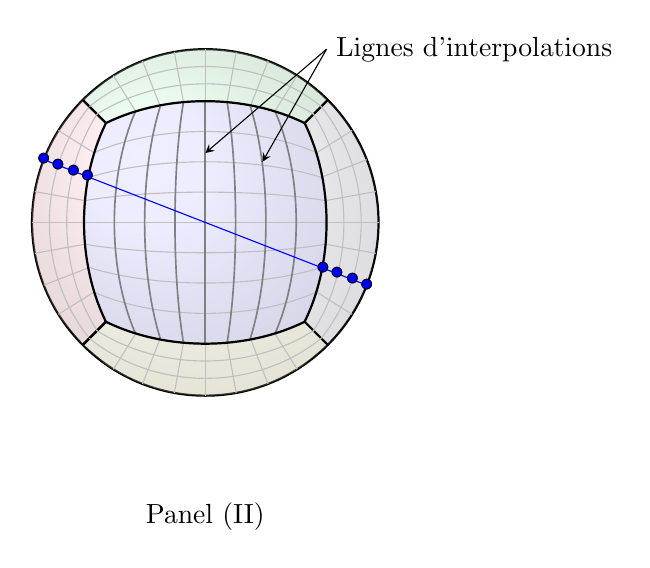
\begin{tikzpicture}[scale=2.2]
	\draw [line width=0.8pt] (0,0) circle (1cm);
    \shade[ball color=blue!10!white,opacity=0.20] (0,0) circle (1cm);	
	
	\filldraw[draw=black,fill=blue!30!white,opacity=0.20]
	plot [smooth,domain=-35:35] ({0.7*cos(\x)},{sin(\x)})
	-- plot [smooth,domain=55:125] ({cos(\x)},{0.7*sin(\x)})
	-- plot [smooth,domain=150:215] ({0.7*cos(\x)},{sin(\x)})
	-- plot [smooth,domain=240:300] ({cos(\x)},{0.7*sin(\x)})
	-- cycle;	
	\draw [samples=100,domain=48:132, color=gray!50] plot({cos(\x)},{0.35*sin(\x)});
	\draw [samples=100,domain=48:132, color=gray!50] plot({cos(\x)},{-.35*sin(\x)});
	\draw [samples=100,domain=46:134, color=gray!50] plot({cos(\x)},{0.175*sin(\x)});
	\draw [samples=100,domain=46:134, color=gray!50] plot({cos(\x)},{-.175*sin(\x)});
	\draw [samples=100,domain=50:130, color=gray!50] plot({cos(\x)},{0.525*sin(\x)});
	\draw [samples=100,domain=50:130, color=gray!50] plot({cos(\x)},{-.525*sin(\x)});
	\draw [samples=100,domain=45:135, color=gray!50] plot({cos(\x)},{0*sin(\x)});

	\draw [rotate=90, samples=100,domain=48:132, color=gray, line width=0.6pt] plot({cos(\x)},{0.35*sin(\x)});
	\draw [rotate=90, samples=100,domain=48:132, color=gray, line width=0.6pt] plot({cos(\x)},{-.35*sin(\x)});
	\draw [rotate=90, samples=100,domain=46:134, color=gray, line width=0.6pt] plot({cos(\x)},{0.175*sin(\x)});
	\draw [rotate=90, samples=100,domain=46:134, color=gray, line width=0.6pt] plot({cos(\x)},{-.175*sin(\x)});
	\draw [rotate=90, samples=100,domain=50:130, color=gray, line width=0.6pt] plot({cos(\x)},{0.525*sin(\x)});
	\draw [rotate=90, samples=100,domain=50:130, color=gray, line width=0.6pt] plot({cos(\x)},{-.525*sin(\x)});
	\draw [rotate=90, samples=100,domain=45:135, color=gray, line width=0.6pt] plot({cos(\x)},{0*sin(\x)});

	\filldraw[draw=black,fill=red!30!white,opacity=0.20]
	plot [smooth,domain=145:215] ({.7*cos(\x)},{sin(\x)})
	-- plot [smooth] (-.573,-.573) -- (-.707,-.707)
	-- plot [smooth,domain=215:145] ({cos(\x)},{sin(\x)})
	-- plot [smooth] (-.707,.707) -- (-.573,.573)
	-- cycle;	
	\draw [line width=0.8pt] (-.573,-.573) -- (-.707,-.707) ;
	\draw [line width=0.8pt] (-.573,.573) -- (-.707,.707) ;
	\draw [color=gray!50] (-.669,.260) -- (-.9321,.3622) ;
	\draw [color=gray!50] (-.669,-.260) -- (-.9321,-.3622) ;
	\draw [color=gray!50] (-.6946,.1259) -- (-.9840,.1783) ;
	\draw [color=gray!50] (-.6946,-.1259) -- (-.9840,-.1783) ;
	\draw [color=gray!50] (-.6427,.4022) -- (-.8477,.5305) ;
	\draw [color=gray!50] (-.6427,-.4022) -- (-.8477,-.5305) ;
	\draw [color=gray!50] (-.707,0) -- (-1,0) ;
	\draw [samples=100,domain=141:219, color=gray!50] plot({0.8*cos(\x)},{sin(\x)});
	\draw [samples=100,domain=138:222, color=gray!50] plot({0.9*cos(\x)},{sin(\x)});
	
	\filldraw[draw=black,fill=green!30!white,opacity=0.20]
	plot [smooth,domain=55:125] ({cos(\x)},{0.7*sin(\x)})
	-- plot [smooth] (-.573,.573) -- (-.707,.707)
	-- plot [smooth,domain=125:55] ({cos(\x)},{sin(\x)})
	-- plot [smooth] (.707,.707) -- (.573,.573)
	-- cycle;	
	\draw [line width=0.8pt] (-.573,.573) -- (-.707,.707) ;
	\draw [line width=0.8pt] (.707,.707) -- (.573,.573) ;
	\draw [rotate=-90,color=gray!50] (-.669,.260) -- (-.9321,.3622) ;
	\draw [rotate=-90,color=gray!50] (-.669,-.260) -- (-.9321,-.3622) ;
	\draw [rotate=-90,color=gray!50] (-.6946,.1259) -- (-.9840,.1783) ;
	\draw [rotate=-90,color=gray!50] (-.6946,-.1259) -- (-.9840,-.1783) ;
	\draw [rotate=-90,color=gray!50] (-.6427,.4022) -- (-.8477,.5305) ;
	\draw [rotate=-90,color=gray!50] (-.6427,-.4022) -- (-.8477,-.5305) ;
	\draw [rotate=-90,color=gray!50] (-.707,0) -- (-1,0) ;
	\draw [rotate=-90,samples=100,domain=141:219, color=gray!50] plot({0.8*cos(\x)},{sin(\x)});
	\draw [rotate=-90,samples=100,domain=138:222, color=gray!50] plot({0.9*cos(\x)},{sin(\x)});
	
	\filldraw[draw=black,fill=yellow!30!white,opacity=0.20]
	plot [smooth,domain=55:125] ({cos(\x)},{-.7*sin(\x)})
	-- plot [smooth] (-.573,-.573) -- (-.707,-.707)
	-- plot [smooth,domain=125:55] ({cos(\x)},{-sin(\x)})
	-- plot [smooth] (.707,-.707) -- (.573,-.573)
	-- cycle;	
	\draw [line width=0.8pt] (-.573,-.573) -- (-.707,-.707) ;
	\draw [line width=0.8pt] (.707,-.707) -- (.573,-.573) ;
	\draw [rotate=90,color=gray!50] (-.669,.260) -- (-.9321,.3622) ;
	\draw [rotate=90,color=gray!50] (-.669,-.260) -- (-.9321,-.3622) ;
	\draw [rotate=90,color=gray!50] (-.6946,.1259) -- (-.9840,.1783) ;
	\draw [rotate=90,color=gray!50] (-.6946,-.1259) -- (-.9840,-.1783) ;
	\draw [rotate=90,color=gray!50] (-.6427,.4022) -- (-.8477,.5305) ;
	\draw [rotate=90,color=gray!50] (-.6427,-.4022) -- (-.8477,-.5305) ;
	\draw [rotate=90,color=gray!50] (-.707,0) -- (-1,0) ;
	\draw [rotate=90,samples=100,domain=141:219, color=gray!50] plot({0.8*cos(\x)},{sin(\x)});
	\draw [rotate=90,samples=100,domain=138:222, color=gray!50] plot({0.9*cos(\x)},{sin(\x)});
	
	\draw [rotate=180,color=gray!50] (-.669,.260) -- (-.9321,.3622) ;
	\draw [rotate=180,color=gray!50] (-.669,-.260) -- (-.9321,-.3622) ;
	\draw [rotate=180,color=gray!50] (-.6946,.1259) -- (-.9840,.1783) ;
	\draw [rotate=180,color=gray!50] (-.6946,-.1259) -- (-.9840,-.1783) ;
	\draw [rotate=180,color=gray!50] (-.6427,.4022) -- (-.8477,.5305) ;
	\draw [rotate=180,color=gray!50] (-.6427,-.4022) -- (-.8477,-.5305) ;
	\draw [rotate=180,color=gray!50] (-.707,0) -- (-1,0) ;
	\draw [rotate=180,samples=100,domain=141:219, color=gray!50] plot({0.8*cos(\x)},{sin(\x)});
	\draw [rotate=180,samples=100,domain=138:222, color=gray!50] plot({0.9*cos(\x)},{sin(\x)});
	
	\draw [samples=100,domain=55:125, line width=0.8pt] plot({cos(\x)},{0.7*sin(\x)});
	\draw [samples=100,domain=55:125, line width=0.8pt] plot({cos(\x)},{-.7*sin(\x)});
	\draw [samples=100,domain=145:215, line width=0.8pt] plot({.7*cos(\x)},{sin(\x)}); 
	\draw [samples=100,domain=145:215, line width=0.8pt] plot({-.7*cos(\x)},{sin(\x)}); 
	
	\draw [color=blue] (-.9321,.3622) -- (.9321,-.3622) ;
	\draw  (-.9321,.3622) node[color=blue] {$\bullet$} ;
	\draw (-.9321,.3622) node {$\circ$} ;	
	\draw  (.9321,-.3622) node[color=blue] {$\bullet$} ;
	\draw (.9321,-.3622) node {$\circ$} ;
	\draw  (-.85,0.3886*.85) node[color=blue] {$\bullet$} ;
	\draw (-.85,0.3886*.85) node {$\circ$} ;	
	\draw (.85,-0.3886*.85) node[color=blue] {$\bullet$} ;
	\draw (.85,-0.3886*.85) node {$\circ$} ;	
	\draw  (-.76,0.3886*.76) node[color=blue] {$\bullet$} ;
	\draw (-.76,0.3886*.76) node {$\circ$} ;	
	\draw (.76,-0.3886*.76) node[color=blue] {$\bullet$} ;
	\draw (.76,-0.3886*.76) node {$\circ$} ;
	\draw  (-.68,0.3886*.68) node[color=blue] {$\bullet$} ;
	\draw (-.68,0.3886*.68) node {$\circ$} ;	
	\draw (.68,-0.3886*.68) node[color=blue] {$\bullet$} ;
	\draw (.68,-0.3886*.68) node {$\circ$} ;	
	\draw (-.52,0.3886*.52) node[color=blue] {\begin{tiny}$\blacksquare$ \end{tiny}} ;
	\draw (-.52,0.3886*.52) node {\begin{tiny}$\square$ \end{tiny}} ;
	\draw (.52,-0.3886*.52) node[color=blue] {\begin{tiny}$\blacksquare$ \end{tiny}} ;
	\draw (.52,-0.3886*.52) node {\begin{tiny}$\square$ \end{tiny}} ;
	\draw (-.36,0.3886*.36) node[color=blue] {\begin{tiny}$\blacksquare$ \end{tiny}} ;
	\draw (-.36,0.3886*.36) node {\begin{tiny}$\square$ \end{tiny}} ;
	\draw (.36,-0.3886*.36) node[color=blue] {\begin{tiny}$\blacksquare$ \end{tiny}} ;
	\draw (.36,-0.3886*.36) node {\begin{tiny}$\square$ \end{tiny}} ;
	\draw (-.18,0.3886*.18) node[color=blue] {\begin{tiny}$\blacksquare$ \end{tiny}} ;
	\draw (-.18,0.3886*.18) node {\begin{tiny}$\square$ \end{tiny}} ;
	\draw (.18,-0.3886*.18) node[color=blue] {\begin{tiny}$\blacksquare$ \end{tiny}} ;
	\draw (.18,-0.3886*.18) node {\begin{tiny}$\square$ \end{tiny}} ;
	\draw (0,0) node[color=blue] {\begin{tiny}$\blacksquare$ \end{tiny}} ;
	\draw (0,0) node {\begin{tiny}$\square$ \end{tiny}} ;
	
	\draw [>=stealth, <-] (.33,.35) -- (.7,1) ;
	\draw [>=stealth, <-] (0,.4) -- (.7,1) ;
	\draw  (0.7,1) node[right] {Lignes d'interpolations} ;
	
	\draw  (0,-1.7) node {Panel (II)} ;

\end{tikzpicture}
\end{center}
\caption{La ligne bleue représente une isoligne $\eta=\eta_j$ du panel $(I)$ vue depuis le panel $(II)$. les cercles bleus représentent des points de la Cubed-Sphere contenues dans l'isoligne $\eta=\eta_j$, les carrés bleus sont des points de l'isoligne $\eta=\eta_j$ qui ne sont pas sur la Cubed-Sphere.}
\label{fig: panel II_interp}
\end{figure}  

La périodicité sur les grands cercles permet d'assurer que $\mathbf{m}_p = \mathbf{m}_{p+4N}$ pour tout $p \in \mathbb{Z}$. De plus, la construction de la Cubed-Sphere, permet d'assurer un paramétrage du grand cercle $C^{(2)}_j$. Chaque point est associé à des coordonnées $(\xi_p, \eta_p)$. Les valeurs de $\xi_p$ donnent un paramétrage des points $\mathbf{m}_p$ le long du grand cercle. On a de plus
\begin{equation}
\xi_{p+1} = \xi_p + \Delta \xi
\end{equation}
Si $f_p = f(\mathbf{m}_p)$ est connue pour tout $p$ vérifiant $0 \leq p \leq 4N-1$ alors on peut calculer la dérivée approchée $f_{\xi,i,j}^k$ de $\partial_{\xi}f(\mathbf{x}_{i,j}^k)$ à l'ordre $4$ grâce à la formule de dérivation hermitienne \eqref{def:herm_4}
\begin{equation}
f_{\xi,i,j}^k = \delta_{\xi}^H f_p.
\end{equation}
Cependant, les valeurs de $f_p$ ne sont pas toutes connues car les points $\mathbf{m}_p$ ne sont pas des points du maillages lorsque $N+1 \leq p \leq 2N-1$ ou $3N+4 \leq p \leq 4N-1$. Il faut donc construire un procéder permettant d'obtenir des valeurs en ces points. Le procédé utilisé dans ce travail est basé sur une interpolation à l'aide de Splines Cubiques.

On souhaite calculer une valeur $f_p$ approchant $f(\mathbf{m}_p)$ avec $N+1 \leq p \leq 2N-1$ ou $3N+4 \leq p \leq 4N-1$. Dans ce cadre, $\mathbf{m}_p$ n'est pas un point de la Cubed-Sphere. Cependant on sait que 
\begin{equation}
\mathbf{m}_p \in C^{(2)}_j \cap C
\end{equation} 
où $C^{(2)}_j$ est une isoligne pour $\eta = \eta_j$ constant pour le panel $(I)$ et $C$ est une isoligne $\xi$ constant pour le panel $(II)$ (si $N+1 \leq p \leq 2N-1$) ou pour le panel $(IV)$ si $3N+4 \leq p \leq 4N-1$ (lignes en gras sur les figures \ref{fig:patron_cs}.et \ref{fig: panel II_interp}).
La méthode consiste à utiliser les points de la Cubed-Sphere présents sur le cercle $C$ pour construire une fonction d'interpolation de type Spline Cubique puis d'évaluer cette fonction au point du maillage $\mathbf{m}_p$. Si on note $P_C$ la fonction d'interpolation en question, on a alors $f_p = P_C (\mathbf{m}_p)$. L'interpolation s'effectuant sur un grand cercle, il s'agit d'une fonction d'interpolation 1D. De plus, cette fonction étant issue des splines cubiques, on a :
\begin{equation}
f_p = P_C(\mathbf{m}_p) = f(\mathbf{m}_p) + \mathcal{O}(\Delta \eta^4).
\end{equation}
La fonction $P_C$ ne dépend pas du point $\mathbf{m}_p$ mais uniquement des données aux points de la Cubed-Sphere sur le panel choisit et le long de $C$ (Voir figure \ref{fig: panel II_interp2}).

\begin{figure}[htbp]
\begin{center}
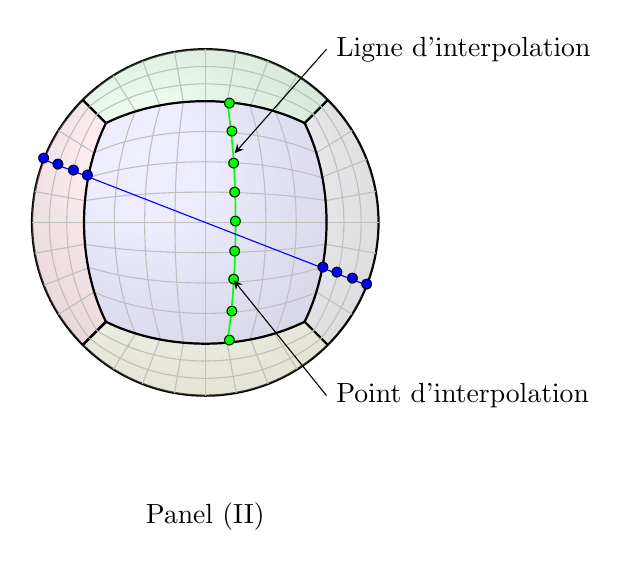
\begin{tikzpicture}[scale=2.2]
	\draw [line width=0.8pt] (0,0) circle (1cm);
    \shade[ball color=blue!10!white,opacity=0.20] (0,0) circle (1cm);	
	
	\filldraw[draw=black,fill=blue!30!white,opacity=0.20]
	plot [smooth,domain=-35:35] ({0.7*cos(\x)},{sin(\x)})
	-- plot [smooth,domain=55:125] ({cos(\x)},{0.7*sin(\x)})
	-- plot [smooth,domain=150:215] ({0.7*cos(\x)},{sin(\x)})
	-- plot [smooth,domain=240:300] ({cos(\x)},{0.7*sin(\x)})
	-- cycle;	
	\draw [samples=100,domain=48:132, color=gray!50] plot({cos(\x)},{0.35*sin(\x)});
	\draw [samples=100,domain=48:132, color=gray!50] plot({cos(\x)},{-.35*sin(\x)});
	\draw [samples=100,domain=46:134, color=gray!50] plot({cos(\x)},{0.175*sin(\x)});
	\draw [samples=100,domain=46:134, color=gray!50] plot({cos(\x)},{-.175*sin(\x)});
	\draw [samples=100,domain=50:130, color=gray!50] plot({cos(\x)},{0.525*sin(\x)});
	\draw [samples=100,domain=50:130, color=gray!50] plot({cos(\x)},{-.525*sin(\x)});
	\draw [samples=100,domain=45:135, color=gray!50] plot({cos(\x)},{0*sin(\x)});

	\draw [rotate=90, samples=100,domain=48:132, color=gray!50] plot({cos(\x)},{0.35*sin(\x)});
	\draw [rotate=90, samples=100,domain=48:132, color=gray!50] plot({cos(\x)},{-.35*sin(\x)});
	\draw [rotate=90, samples=100,domain=46:134, color=green, line width=0.6pt] plot({cos(\x)},{-.175*sin(\x)});
	\draw [rotate=90, samples=100,domain=46:134, color=gray!50] plot({cos(\x)},{0.175*sin(\x)});
	\draw [rotate=90, samples=100,domain=50:130, color=gray!50] plot({cos(\x)},{0.525*sin(\x)});
	\draw [rotate=90, samples=100,domain=50:130, color=gray!50] plot({cos(\x)},{-.525*sin(\x)});
	\draw [rotate=90, samples=100,domain=45:135, color=gray!50] plot({cos(\x)},{0*sin(\x)});

	\filldraw[draw=black,fill=red!30!white,opacity=0.20]
	plot [smooth,domain=145:215] ({.7*cos(\x)},{sin(\x)})
	-- plot [smooth] (-.573,-.573) -- (-.707,-.707)
	-- plot [smooth,domain=215:145] ({cos(\x)},{sin(\x)})
	-- plot [smooth] (-.707,.707) -- (-.573,.573)
	-- cycle;	
	\draw [line width=0.8pt] (-.573,-.573) -- (-.707,-.707) ;
	\draw [line width=0.8pt] (-.573,.573) -- (-.707,.707) ;
	\draw [color=gray!50] (-.669,.260) -- (-.9321,.3622) ;
	\draw [color=gray!50] (-.669,-.260) -- (-.9321,-.3622) ;
	\draw [color=gray!50] (-.6946,.1259) -- (-.9840,.1783) ;
	\draw [color=gray!50] (-.6946,-.1259) -- (-.9840,-.1783) ;
	\draw [color=gray!50] (-.6427,.4022) -- (-.8477,.5305) ;
	\draw [color=gray!50] (-.6427,-.4022) -- (-.8477,-.5305) ;
	\draw [color=gray!50] (-.707,0) -- (-1,0) ;
	\draw [samples=100,domain=141:219, color=gray!50] plot({0.8*cos(\x)},{sin(\x)});
	\draw [samples=100,domain=138:222, color=gray!50] plot({0.9*cos(\x)},{sin(\x)});
	
	\filldraw[draw=black,fill=green!30!white,opacity=0.20]
	plot [smooth,domain=55:125] ({cos(\x)},{0.7*sin(\x)})
	-- plot [smooth] (-.573,.573) -- (-.707,.707)
	-- plot [smooth,domain=125:55] ({cos(\x)},{sin(\x)})
	-- plot [smooth] (.707,.707) -- (.573,.573)
	-- cycle;	
	\draw [line width=0.8pt] (-.573,.573) -- (-.707,.707) ;
	\draw [line width=0.8pt] (.707,.707) -- (.573,.573) ;
	\draw [rotate=-90,color=gray!50] (-.669,.260) -- (-.9321,.3622) ;
	\draw [rotate=-90,color=gray!50] (-.669,-.260) -- (-.9321,-.3622) ;
	\draw [rotate=-90,color=gray!50] (-.6946,.1259) -- (-.9840,.1783) ;
	\draw [rotate=-90,color=gray!50] (-.6946,-.1259) -- (-.9840,-.1783) ;
	\draw [rotate=-90,color=gray!50] (-.6427,.4022) -- (-.8477,.5305) ;
	\draw [rotate=-90,color=gray!50] (-.6427,-.4022) -- (-.8477,-.5305) ;
	\draw [rotate=-90,color=gray!50] (-.707,0) -- (-1,0) ;
	\draw [rotate=-90,samples=100,domain=141:219, color=gray!50] plot({0.8*cos(\x)},{sin(\x)});
	\draw [rotate=-90,samples=100,domain=138:222, color=gray!50] plot({0.9*cos(\x)},{sin(\x)});
	
	\filldraw[draw=black,fill=yellow!30!white,opacity=0.20]
	plot [smooth,domain=55:125] ({cos(\x)},{-.7*sin(\x)})
	-- plot [smooth] (-.573,-.573) -- (-.707,-.707)
	-- plot [smooth,domain=125:55] ({cos(\x)},{-sin(\x)})
	-- plot [smooth] (.707,-.707) -- (.573,-.573)
	-- cycle;	
	\draw [line width=0.8pt] (-.573,-.573) -- (-.707,-.707) ;
	\draw [line width=0.8pt] (.707,-.707) -- (.573,-.573) ;
	\draw [rotate=90,color=gray!50] (-.669,.260) -- (-.9321,.3622) ;
	\draw [rotate=90,color=gray!50] (-.669,-.260) -- (-.9321,-.3622) ;
	\draw [rotate=90,color=gray!50] (-.6946,.1259) -- (-.9840,.1783) ;
	\draw [rotate=90,color=gray!50] (-.6946,-.1259) -- (-.9840,-.1783) ;
	\draw [rotate=90,color=gray!50] (-.6427,.4022) -- (-.8477,.5305) ;
	\draw [rotate=90,color=gray!50] (-.6427,-.4022) -- (-.8477,-.5305) ;
	\draw [rotate=90,color=gray!50] (-.707,0) -- (-1,0) ;
	\draw [rotate=90,samples=100,domain=141:219, color=gray!50] plot({0.8*cos(\x)},{sin(\x)});
	\draw [rotate=90,samples=100,domain=138:222, color=gray!50] plot({0.9*cos(\x)},{sin(\x)});
	
	\draw [rotate=180,color=gray!50] (-.669,.260) -- (-.9321,.3622) ;
	\draw [rotate=180,color=gray!50] (-.669,-.260) -- (-.9321,-.3622) ;
	\draw [rotate=180,color=gray!50] (-.6946,.1259) -- (-.9840,.1783) ;
	\draw [rotate=180,color=gray!50] (-.6946,-.1259) -- (-.9840,-.1783) ;
	\draw [rotate=180,color=gray!50] (-.6427,.4022) -- (-.8477,.5305) ;
	\draw [rotate=180,color=gray!50] (-.6427,-.4022) -- (-.8477,-.5305) ;
	\draw [rotate=180,color=gray!50] (-.707,0) -- (-1,0) ;
	\draw [rotate=180,samples=100,domain=141:219, color=gray!50] plot({0.8*cos(\x)},{sin(\x)});
	\draw [rotate=180,samples=100,domain=138:222, color=gray!50] plot({0.9*cos(\x)},{sin(\x)});
	
	\draw [samples=100,domain=55:125, line width=0.8pt] plot({cos(\x)},{0.7*sin(\x)});
	\draw [samples=100,domain=55:125, line width=0.8pt] plot({cos(\x)},{-.7*sin(\x)});
	\draw [samples=100,domain=145:215, line width=0.8pt] plot({.7*cos(\x)},{sin(\x)}); 
	\draw [samples=100,domain=145:215, line width=0.8pt] plot({-.7*cos(\x)},{sin(\x)}); 
	
	\draw (.175,0) node[color=green] {$\bullet$} ;
	\draw (.175,0) node {$\circ$} ;
	\draw (.17,.17) node[color=green] {$\bullet$} ;
	\draw (.17,.17) node {$\circ$} ;
	\draw (.165,.335) node[color=green] {$\bullet$} ;
	\draw (.165,.335) node {$\circ$} ;
	\draw (.155,.52) node[color=green] {$\bullet$} ;
	\draw (.155,.52) node {$\circ$} ;
	\draw (.14,.684) node[color=green] {$\bullet$} ;
	\draw (.14,.684) node {$\circ$} ;
	\draw (.17,-.17) node[color=green] {$\bullet$} ;
	\draw (.17,-.17) node {$\circ$} ;
	\draw (.165,-.335) node[color=green] {$\bullet$} ;
	\draw (.165,-.335) node {$\circ$} ;
	\draw (.155,-.52) node[color=green] {$\bullet$} ;
	\draw (.155,-.52) node {$\circ$} ;
	\draw (.14,-.684) node[color=green] {$\bullet$} ;
	\draw (.14,-.684) node {$\circ$} ;
	
	\draw [>=stealth, <-] (0.17,.4) -- (.7,1) ;
	\draw  (0.7,1) node[right] {Ligne d'interpolation} ;
	\draw [>=stealth, <-] (.165,-.335) -- (.7,-1) ;
	\draw  (0.7,-1) node[right] {Point d'interpolation} ;
	
	
	
	
	
	
	\draw [color=blue] (-.9321,.3622) -- (.9321,-.3622) ;
	\draw  (-.9321,.3622) node[color=blue] {$\bullet$} ;
	\draw (-.9321,.3622) node {$\circ$} ;	
	\draw  (.9321,-.3622) node[color=blue] {$\bullet$} ;
	\draw (.9321,-.3622) node {$\circ$} ;
	\draw  (-.85,0.3886*.85) node[color=blue] {$\bullet$} ;
	\draw (-.85,0.3886*.85) node {$\circ$} ;	
	\draw (.85,-0.3886*.85) node[color=blue] {$\bullet$} ;
	\draw (.85,-0.3886*.85) node {$\circ$} ;	
	\draw  (-.76,0.3886*.76) node[color=blue] {$\bullet$} ;
	\draw (-.76,0.3886*.76) node {$\circ$} ;	
	\draw (.76,-0.3886*.76) node[color=blue] {$\bullet$} ;
	\draw (.76,-0.3886*.76) node {$\circ$} ;
	\draw  (-.68,0.3886*.68) node[color=blue] {$\bullet$} ;
	\draw (-.68,0.3886*.68) node {$\circ$} ;	
	\draw (.68,-0.3886*.68) node[color=blue] {$\bullet$} ;
	\draw (.68,-0.3886*.68) node {$\circ$} ;	
	\draw (-.52,0.3886*.52) node[color=blue] {\begin{tiny}$\blacksquare$ \end{tiny}} ;
	\draw (-.52,0.3886*.52) node {\begin{tiny}$\square$ \end{tiny}} ;
	\draw (.52,-0.3886*.52) node[color=blue] {\begin{tiny}$\blacksquare$ \end{tiny}} ;
	\draw (.52,-0.3886*.52) node {\begin{tiny}$\square$ \end{tiny}} ;
	\draw (-.36,0.3886*.36) node[color=blue] {\begin{tiny}$\blacksquare$ \end{tiny}} ;
	\draw (-.36,0.3886*.36) node {\begin{tiny}$\square$ \end{tiny}} ;
	\draw (.36,-0.3886*.36) node[color=blue] {\begin{tiny}$\blacksquare$ \end{tiny}} ;
	\draw (.36,-0.3886*.36) node {\begin{tiny}$\square$ \end{tiny}} ;
	\draw (-.18,0.3886*.18) node[color=blue] {\begin{tiny}$\blacksquare$ \end{tiny}} ;
	\draw (-.18,0.3886*.18) node {\begin{tiny}$\square$ \end{tiny}} ;
	\draw (.18,-0.3886*.18) node[color=blue] {\begin{tiny}$\blacksquare$ \end{tiny}} ;
	\draw (.18,-0.3886*.18) node {\begin{tiny}$\square$ \end{tiny}} ;
	\draw (0,0) node[color=blue] {\begin{tiny}$\blacksquare$ \end{tiny}} ;
	\draw (0,0) node {\begin{tiny}$\square$ \end{tiny}} ;
	
	\draw  (0,-1.7) node {Panel (II)} ;

\end{tikzpicture}
\end{center}
\caption{La ligne bleue représente une isoligne $\eta=\eta_j$ du panel $(I)$ vue depuis le panel $(II)$. les cercles bleus représentent des points de la Cubed-Sphere contenues dans l'isoligne $\eta=\eta_j$, les carrés bleus sont des points de l'isoligne $\eta=\eta_j$ qui ne sont pas sur la Cubed-Sphere. En vert, une portion du grand cercle utilisé pour l'interpolation.}
\label{fig: panel II_interp2}
\end{figure}  

Le procédé est symétrique pour reconstruire les données sur un grand cercle $C_i^{(1)}$ ou le grand cercle d'un autre panel.
Une fois les données $(f_p)_{0 \leq p \leq 4N-1}$ construites, on peut calculer l'approximation de la dérivée grâce à $\partial_{\xi} f_p \approx \delta_{\Delta \xi}^H f_p$
que l'on restreint aux points du maillage par 
\begin{equation}
\left\lbrace
\begin{array}{rcl}
f_{\xi,i,j}^{(I)} & = & \delta_{\Delta \xi}^H f_{i-N/2}\\
f_{\xi,i,j}^{(III)} & = & \delta_{\Delta \xi}^H f_{i+3N/2}
\end{array}
\right.
\text{ pour } C^{(2)}_j \text{ fixé.}
\end{equation}

Finalement, le procédé total de calcul des dérivées hermitienne est $\xi$ sur un panel $k$ est donné par l'algorithme \ref{alg:deltaxi}.

\begin{center}
\begin{minipage}[H]{12cm}
  \begin{algorithm}[H]
    \caption{: Calcul de $f_{\xi, i, j}^{(I)}$ et $f_{\xi, i, j}^{(III)}$}\label{alg:deltaxi}
    \begin{algorithmic}[1]
    \For{ $j=-N/2, \ldots , N/2$, }
    \State pour un grand cercle $C_j^{(2)}$ fixé,
    \For{$p=0,1, \ldots 4N-1$ définir les points $\mathbf{m}_p$ du grand cercle bleu}
             \State  $\mathbf{m}_p = \mathbf{m}_{p-N/2,j}^{(I)}$ pour $0  \leq p \leq N$ donc $f_p = f(\mathbf{m}_p)$,
             \State $f_p = P_{C_p}(\mathbf{m}_p)$, où $P_{C_p}$ est la fonction d'interpolation utilisant les points de l'isoligne $\xi = \xi^{(II)}_{p-N/2+1}$ pour $N+1 \leq p \leq 2N-1$,
             \State  $\mathbf{m}_p = \mathbf{m}_{p-3N/2,j}^{(III)}$ pour $2N  \leq p \leq 3N-1$ donc $f_p = f(\mathbf{m}_p)$,
             \State $f_p = P_{C_p}(\mathbf{m}_p)$, où $P_{C_p}$ est la fonction d'interpolation utilisant les points de l'isoligne $\xi = \xi^{(VI)}_{p-3N/2+1}$ pour $3N+1 \leq p \leq 4N-1$.
            \EndFor
    \State Calcul de $\delta_{\Delta \xi}^H f_p$,
    \State Affectation $f_{\xi,i,j}^{(I)} = \delta_{\Delta \xi}^H f_{i+N/2}$,
    \State Affectation $f_{\xi,i,j}^{(III)} = \delta_{\Delta \xi}^H f_{i+3N/2}$.
    \EndFor
    \end{algorithmic}
    \end{algorithm}
\end{minipage}
\end{center}
De la même manière, l'algorithme de construction des dérivées approchées en $\eta$ sur les panels $(I)$ et $(III)$ est l'algorithme \ref{alg:deltaeta}.
\begin{center}
\begin{minipage}[H]{12cm}
  \begin{algorithm}[H]
    \caption{: Calcul de $f_{\eta, i, j}^{(I)}$ et $f_{\eta, i, j}^{(III)}$}\label{alg:deltaeta}
    \begin{algorithmic}[1]
    \For{ $i=-N/2, \ldots , N/2$, }
    \State pour un grand cercle $C_i^{(1)}$ fixé,
    \For{$p=0,1, \ldots 4N-1$ définir les points $\mathbf{m}_p$}
             \State  $\mathbf{m}_p = \mathbf{m}_{i,p-N/2}^{(I)}$ pour $0  \leq p \leq N$ donc $f_p = f(\mathbf{m}_p)$,
             \State $f_p = P_{C_p}(\mathbf{m}_p)$, où $P_{C_p}$ est la fonction d'interpolation utilisant les points de l'isoligne $\eta = \eta^{(V)}_{p-N/2+1}$ pour $N+1 \leq p \leq 2N-1$,
             \State  $\mathbf{m}_p = \mathbf{m}_{i,5N/2-p}^{(III)}$ pour $2N  \leq p \leq 3N-1$ donc $f_p = f(\mathbf{m}_p)$ (Attention à l'orientation sur les panels),
             \State $f_p = P_{C_p}(\mathbf{m}_p)$, où $P_{C_p}$ est la fonction d'interpolation utilisant les points de l'isoligne $\eta = \eta^{(VI)}_{p-3N/2+1}$ pour $3N+1 \leq p \leq 4N-1$.
            \EndFor
    \State Calcul de $\delta_{\Delta \eta}^H f_p$,
    \State Affectation $f_{\eta,i,j}^{(I)} = \delta_{\Delta \xi}^H f_{i+N/2}$,
    \State Affectation $f_{\eta,i,j}^{(III)} = \delta_{\Delta \xi}^H f_{i+3N/2}$.
    \EndFor
    \end{algorithmic}
    \end{algorithm}
\end{minipage}
\end{center}
Le processus est utilisé sur chaque panel $(k) = (I), \ldots , (VI)$. On obtient alors les approximations des dérivées en $\xi$ et en $\eta$ sur chaque point du maillage Cubed-Sphere $\mathbf{x}_{i,j}^{(k)}$ avec $-N/2 \leq i,j \leq N/2$.

\begin{theoreme}
Pour tous $-N/2 \leq i,j \leq N/2$ et $(k) = (I) , \ldots , (VI)$ et pour $f : \mathbf{x} \in \mathbb{S}_a^2 \mapsto f(\mathbf{x}) \in \mathbb{R}$ une fonction régulière, on a 
\begin{equation}
\left\lbrace
\begin{array}{rcl}
f_{\xi,i,j}^{(k)} & = & \partial_{\xi} f(\mathbf{x}_{i,j}^{(k)}) + \mathcal{O}(\Delta \eta^3) \\
f_{\eta,i,j}^{(k)} & = & \partial_{\eta} f(\mathbf{x}_{i,j}^{(k)}) + \mathcal{O}(\Delta \xi^3)
\end{array}
\right.
\end{equation}
\label{th:consistance_der_xieta}
\end{theoreme}

\begin{proof}
La preuve est la même sur chaque panel, on se concentre ici sur le panel $(I)$. De plus, par symétrie, nous ne montrons que le premier résultat :
\begin{equation}
f_{\xi,i,j}^{(k)} = \partial_{\xi} f(\mathbf{x}_{i,j}^{(k)}) + \mathcal{O}(\Delta \eta^3)
\end{equation}
Le procédé de construction des valeur sur un grand cercle $C_j^{(2)}$, aux points $\mathbf{m}_p$ avec $0 \leq p \leq 4N-1$, nous donne le résultat
\begin{equation}
f_p = f(\mathbf{m}_p) + \mathcal{O}(\Delta \eta^4)
\end{equation}
Donc dans le calcul effectif de la dérivée Hermitienne, on a 
\begin{equation}
\delta_{\xi} f_p = \dfrac{f_{p+1} - f_{p-1}}{2 \Delta \xi} = \dfrac{f(\mathbf{m}_{p+1}) - f(\mathbf{m}_{p-1})}{2 \Delta \xi} + \mathcal{O}\left( \dfrac{\Delta \eta^4}{\Delta \xi} \right).
\end{equation}
On considère que sur la Cubed-Sphere $\Delta \xi = \Delta \eta$. Alors en composant par $\sigma_{\xi}^{-1}$, on a 
\begin{align*}
\delta_{\xi}^H f_p & = \sigma_{\xi}^{-1} \circ \delta_{\xi} f_p \\
                   & = \sigma_{\xi}^{-1} \circ \left( \dfrac{f(\mathbf{m}_{p+1}) - f(\mathbf{m}_{p-1})}{2 \Delta \xi} + \mathcal{O}\left( \Delta \eta^3 \right) \right)\\
                   & = \sigma_{\xi}^{-1} \circ \left( \dfrac{f(\mathbf{m}_{p+1}) - f(\mathbf{m}_{p-1})}{2 \Delta \xi}\right)  + \mathcal{O}\left( \Delta \eta^3 \right) \\
                   & = \partial_{\xi}f(\mathbf{m}_p) + \mathcal{O}\left( \Delta \eta^3 \right) + \mathcal{O}\left( \Delta \xi^4 \right) \\
                   & = \partial_{\xi}f(\mathbf{m}_p) + \mathcal{O}\left( \Delta \eta^3 \right).\\
\end{align*}
On assigne les dérivées aux points des panels à l'aide de $\mathbf{m}_p=\mathbf{x}^{(k)}_{p-N/2,j}$ pour $p = 0 \ldots N$. Le résultat est alors :
\begin{equation}
f^{(k)}_{\xi,i,j} = \delta_{\xi}^H f_{i+N/2} = \partial_{\xi} f(\mathbf{x}^{(k)}_{i+N/2,j}) + \mathcal{O}\left( \Delta \eta^3 \right).
\end{equation}
Le résultat concernant la dérivée en $\eta$ est obtenu de la même manière.
\end{proof}

D'après le théorème \ref{th:consistance_der_xieta}, la méthode de calcul est d'ordre au moins 3. Cependant, on note que l'interpolation (qui empêche la méthode d'être d'ordre 4) n'intervient qu'en dehors des panels où l'on souhaite calculer la dérivée.
Lorsque l'on souhaite calculer une approximation de $\partial_{\xi}f(\mathbf{x}_{i,j}^{(I)})$, l'interpolation intervient sur les panels $(II)$ et $(IV)$ mais pas sur le panel $(I)$. Dans la pratique, on s'attend à ce que la méthode soit d'ordre $4$, en particulier loin des bords des panels.



\subsection{Opérateur gradient discret}

Soit $h : \mathbf{x} \in \mathbb{S}_a^2 \mapsto h(\mathbf{x}) \in \mathbb{R}$ une fonction régulière sur la Sphère. On note $h_{i,j}^{(k)} = h(\mathbf{x}_{i,j}^{(k)})$, avec $-N/2 \leq i,j \leq N/2$ et $(k) = (I) , \ldots , (VI)$, la valeur de $h$ au point $\mathbf{x}_{i,j}^{(k)}$ de la Cubed-Sphere.
Nous notons $( \mathbf{g}^{\xi} )_{i,j}^{(k)} = \mathbf{g}^{\xi} (\mathbf{x}_{i,j}^{(k)})$ et $( \mathbf{g}^{\eta} )_{i,j}^{(k)} = \mathbf{g}^{\eta} (\mathbf{x}_{i,j}^{(k)})$.

\begin{definition}
On définit l'opérateur \textit{gradient discret} par 
\begin{equation}
\nabla_{T,\Delta} h_{i,j}^{(k)} = h_{\xi,i,j}^{(k)} ( \mathbf{g}^{\xi} )_{i,j}^{(k)} + h_{\eta,i,j}^{(k)} ( \mathbf{g}^{\eta} )_{i,j}^{(k)}
\end{equation}
avec $-N/2 \leq i,j \leq N/2$ et $(k) = (I), \ldots , (VI)$ ainsi que $h_{\xi,i,j}^{(k)}$ et $h_{\eta,i,j}^{(k)}$ obtenus grâce aux algorithmes \ref{alg:deltaxi} et \ref{alg:deltaeta}.
\end{definition}
L'opérateur gradient discret de $h$, $\nabla_{T,\Delta} h_{i,j}^{(k)}$ donne une approximation du gradient continu en $\mathbf{x}_{i,j}^{(k)}$. En effet, le résultat de consistance suivant est vérifié:

\begin{proposition}
Soit $h : \mathbf{x} \in \mathbb{S}_a^2 \mapsto h(\mathbf{x}) \in \mathbb{R}$ une fonction régulière sur la Sphère. Alors, pour tout $-N/2 \leq i,j \leq N/2$ et $(k)=(I), \ldots , (VI)$, on a
\begin{equation}
\nabla_{T,\Delta} h_{i,j}^{(k)} - (\nabla_T h)^{*,(k)}_{i,j} = \mathcal{O} \left( \Delta^3 \right)
\end{equation}
où $^*$ désigne la restriction à la Cubed-Sphere et $\Delta = \Delta \xi = \Delta \eta$. 
\end{proposition}

\begin{proof}
Ce résultat est une conséquence immédiate de la linéarité du gradient discret et du théorème \ref{th:consistance_der_xieta}.
\end{proof}
De plus, on note que par construction
\begin{equation}
\nabla_{T,\Delta} h_{i,j}^{(k)} \in \mathbb{T}_{\mathbf{x}_{i,j}^{(k)}} \mathbb{S}_a^2.
\end{equation}
Une fois l'opérateur d'approximation du gradient définit, il faut le tester numériquement pour tester son comportement. On se donne $h$ tel que le gradient $\nabla_T h$ est connue et nous comparons le gradient approché et le gradient exacte.
Si $h$ est une fonction sphérique, on sait que $h$ se décompose comme une somme d'harmoniques sphériques. De plus, les harmoniques sphériques sont des restrictions de polynômes sur la Sphère $\mathbb{S}_a^2$. Un test pertinent est donc de choisir $h$ de la forme
\begin{equation}
\left\lbrace
\begin{array}{rcl}
\hat{h}(x,y,z) & = & x^p y^q z^r, \\
h & = & \hat{h}_{| \mathbb{S}_a^2}.
\end{array}
\right.
\end{equation}
Avec $p, q, r \in \mathbb{N}$.
En se basant sur la proposition \ref{prop:gradient_project}, on peut facilement déterminer le gradient de $h$ par
\begin{equation}
\nabla_T h = \nabla_{\mathbb{R}^3} \hat{h} - \mathbf{n} \left( \mathbf{n} \cdot \nabla_{\mathbb{R}^3} \hat{h} \right)
\end{equation}
avec $\mathbf{n} = \mathbf{x}/a$ la normale extérieure en $\mathbf{x} \in \mathbb{S}_a^2$ et $\nabla_{\mathbb{R}^3} \hat{h}$ donné dans la base $(\mathbf{i}, \mathbf{j}, \mathbf{k})$ par 
\begin{align*}
\nabla_{\mathbb{R}^3} \hat{h} & = \dfrac{\partial \hat{h}}{\partial x} \mathbf{i} + \dfrac{\partial \hat{h}}{\partial y} \mathbf{j} + \dfrac{\partial \hat{h}}{\partial z} \mathbf{k}\\
                              & = p x^{p-1} y^q z^r \mathbf{i} + q x^p y^{q-1} z^r \mathbf{j} + r x^p y^q z^{r-1} \mathbf{k}.
\end{align*}
Si $\mathbf{u}$ est une fonction vectorielle définit sur la Cubed-Sphere, alors
\begin{equation}
\mathbf{u}_{i,j}^{(k)} = u_{i,j}^{(k)} \mathbf{i} + v_{i,j}^{(k)} \mathbf{j} + w_{i,j}^{(k)} \mathbf{k}
\end{equation}
On définit la norme $\mathcal{N}$ par
\begin{equation}
\mathcal{N}(\mathbf{u}) = \max_{-N/2 \leq i,j \leq N/2} \max_{(k) = (I) \ldots (VI)} \max (u_{i,j}^{(k)}, v_{i,j}^{(k)}, w_{i,j}^{(k)}).
\end{equation}
On mesure l'erreur faite sur le calcul du gradient approché par
\begin{equation}
e_{\Delta} = \dfrac{\mathcal{N}\left(\nabla_{T,\Delta}h - \left( \nabla_{T}h \right)^* \right)}{\mathcal{N}\left(\left( \nabla_{T}h \right)^* \right)}
\end{equation}
Dans la figure \REF, on trace cette erreur en fonction de $\frac{\pi a}{2 N}$.









\subsection{Variante de l'opérateur de gradient discret}


\subsection{Opérateur divergence discret}

\subsection{Variante de l'opérateur de divergence discret}

\subsection{Opérateur rotationnel discret}

\section{Opérateur de filtrage}

\subsection{Définition des opérateurs de filtrage}

\subsection{Filtrage directionnel}

\subsection{Composition des filtrages directionnels}

\subsection{Filtrage numérique}
